\section{Structuur}
\subsection{Leslokalen en vakken}
Volgend UML diagram beschrijft de structuur van de verscheidene klassen betreffende leslokalen en lessen die met elkaar gerelateerd zijn op het logisch niveau van het systeem.
Deze klassen bezitten data vanuit de databank die nodig zullen zijn om lessenroosters en examenroosters te plannen.

\begin{figure}[H]
	\centering
	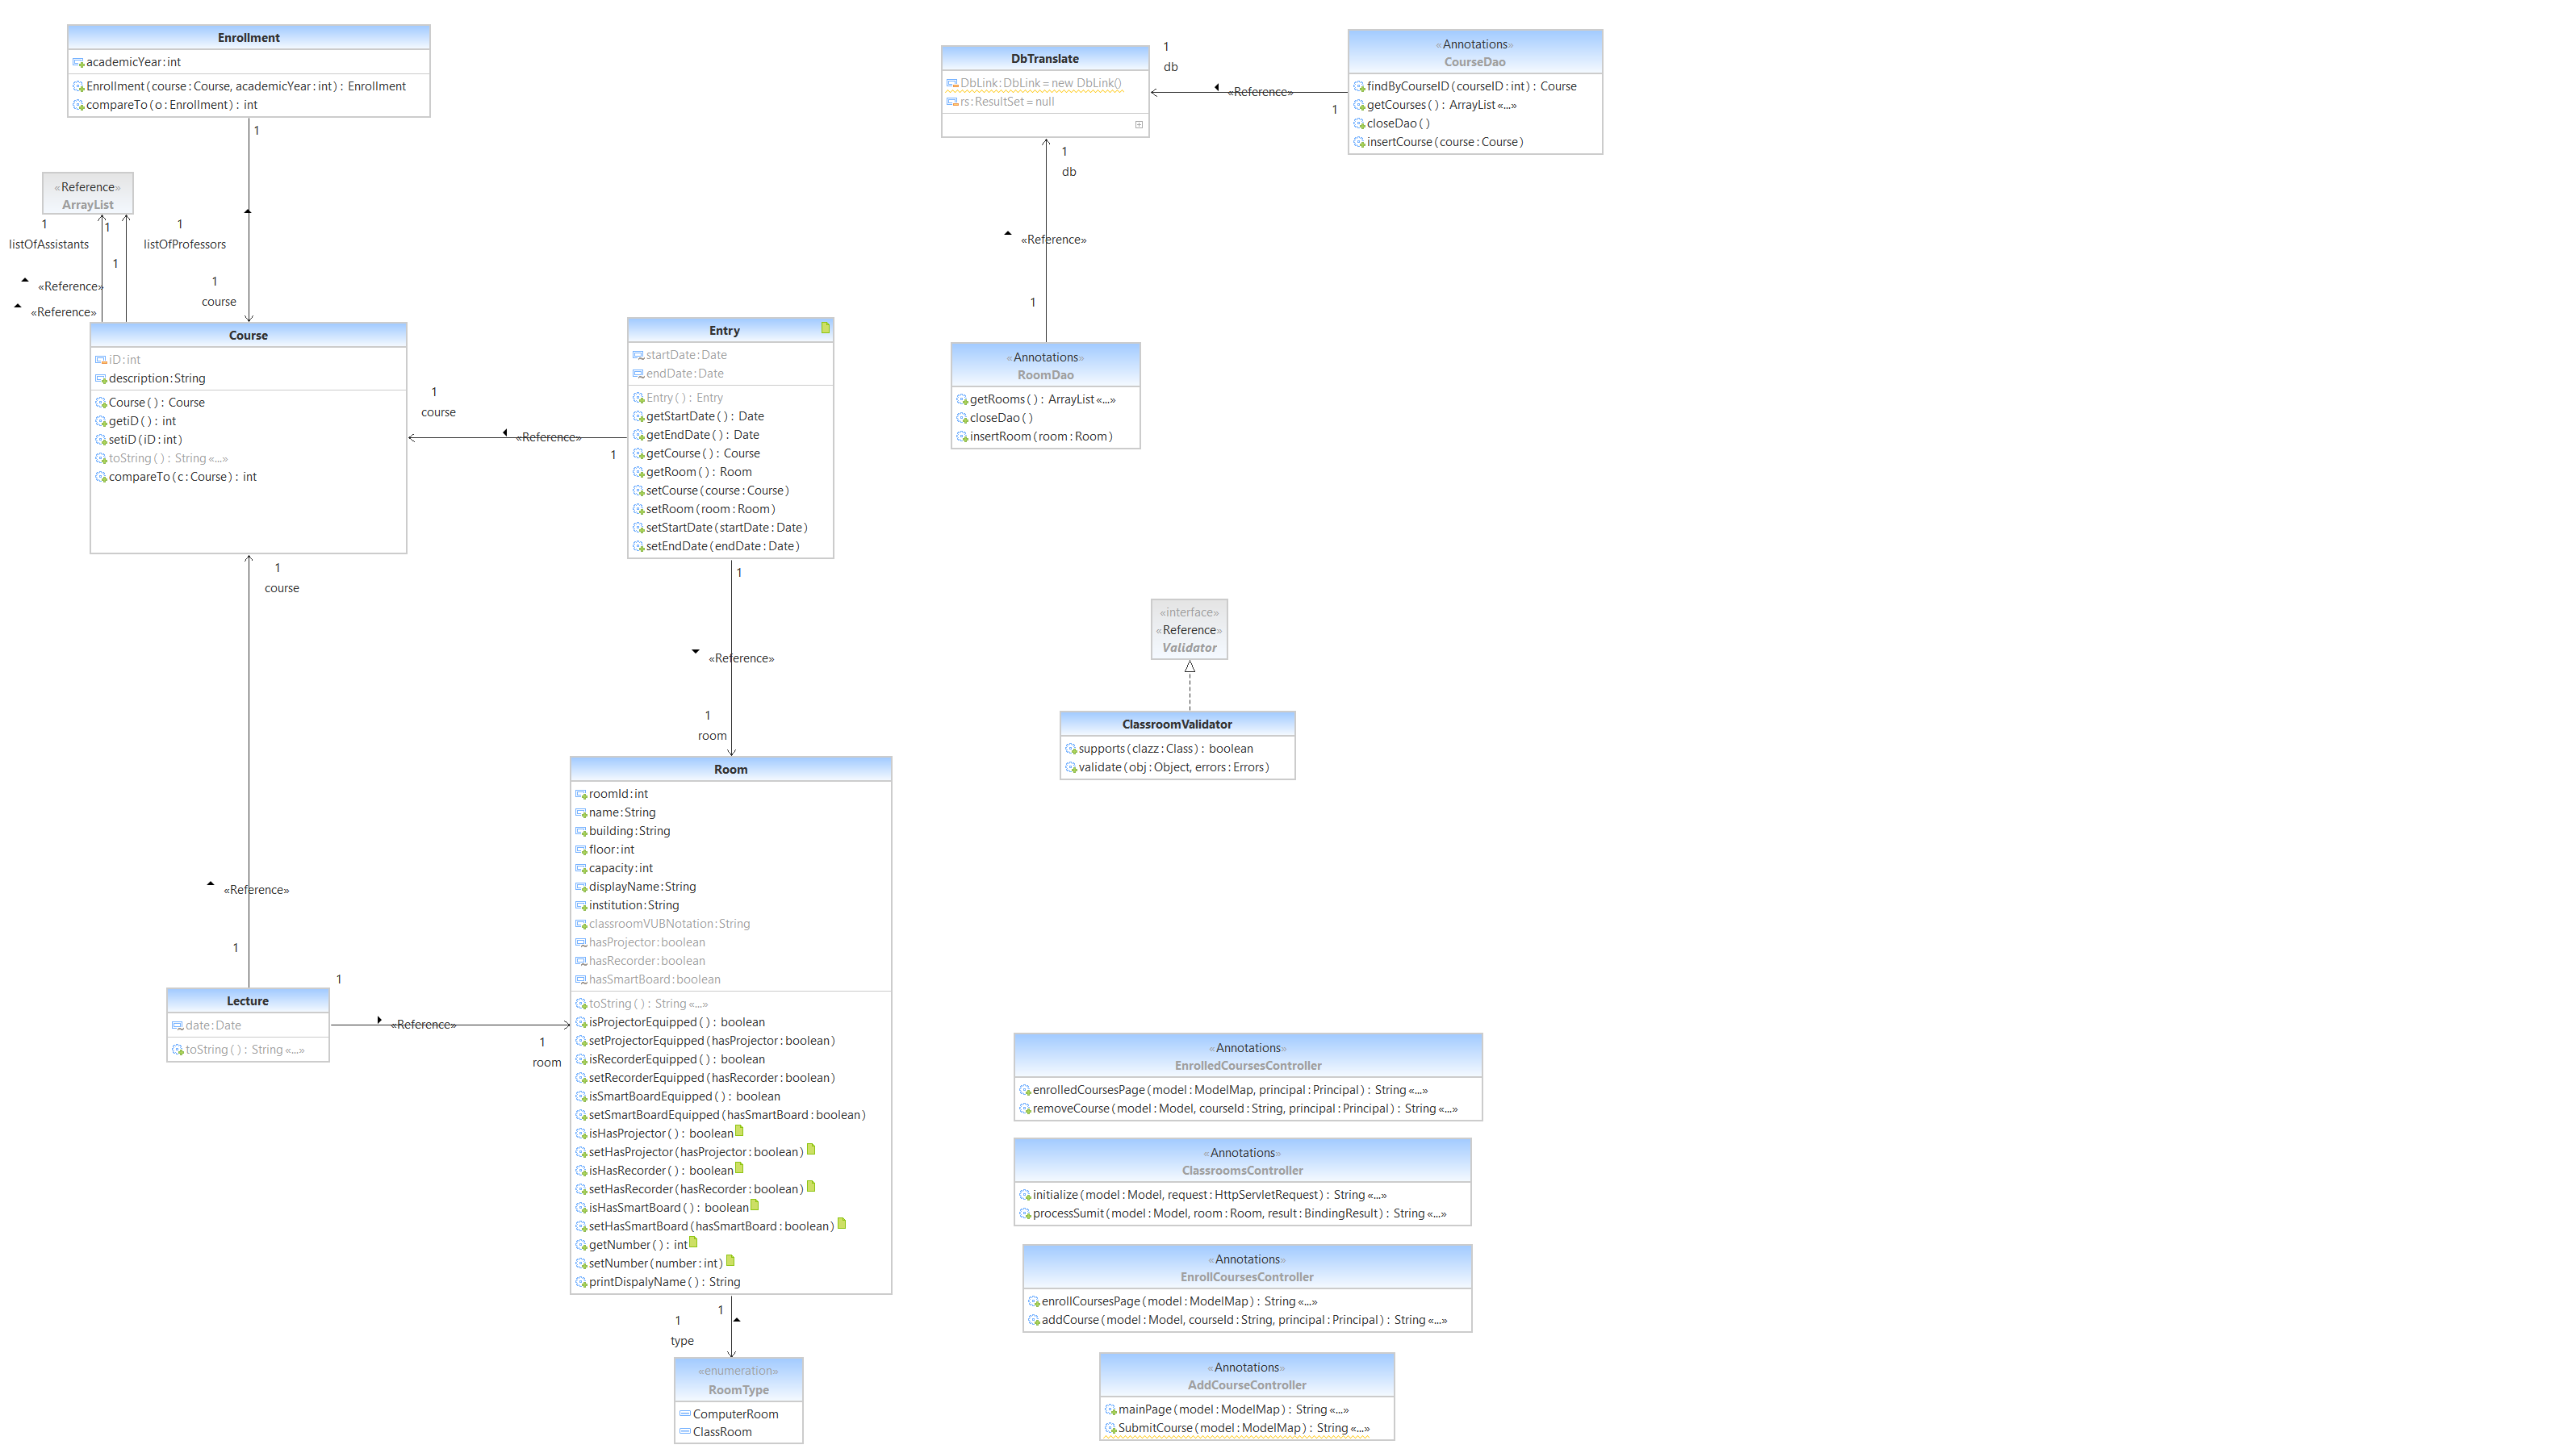
\includegraphics[scale=0.2]{img/roomsAndCourses}
	\caption{UML klassediagram voor leslokalen en vakken}
	\label{fig:roomsAndCourses}
\end{figure}